%%%%%%%%%%%%%%%%%%%%%%%%%%%%%%%%%%%%%%%%%
% University/School Laboratory Report
% LaTeX Template
% Version 2.0 (4/12/12)
%
% This template has been downloaded from:
% http://www.latextemplates.com
%
% License:
% CC BY-NC-SA 3.0 (http://creativecommons.org/licenses/by-nc-sa/3.0/)
%
% Original header:
%
% This is a LaTeX version of the sample laboratory report
% from Virginia Tech's copyrighted 08-09 CHEM 1045/1046 lab manual.
% Reproduction of this one appendix section for academic purposes
% should fall under fair use.
%
%%%%%%%%%%%%%%%%%%%%%%%%%%%%%%%%%%%%%%%%%

\documentclass{article}
\usepackage{graphicx}
\usepackage{mathtools}

\title{ELEC 302-81\\ Lab 1\\ Power in AC Circuits} % Title
% \author{John \textsc{Smith}} % Author name
\date{\today} % Specify a date for the report

\begin{document}

\maketitle

\begin{center}
  \begin{tabular}{l r}
    Date Performed: & January 14, 2013 \\
    Partners: & Rawley Dent \\
    & Charles Pittman \\
    Instructor: & Dr. Weatherford
  \end{tabular}
\end{center}

\pagebreak

\setlength\parindent{0pt} % Removes all indentation from paragraphs

\section{Introduction}
Praesent congue faucibus turpis et cursus. Phasellus vitae nisi felis,
elementum malesuada ante. Aliquam bibendum quam ac libero sollicitudin vel
congue eros feugiat. Aenean ultricies malesuada felis ut vestibulum. Praesent
non tellus risus. Nulla feugiat mauris sed nisl hendrerit ultricies vitae non

Donec non mollis turpis. Etiam tempus ligula et tellus tempus a mollis massa
faucibus. Proin ac interdum risus. Duis nec lacus elit. Donec venenatis
tristique diam, in sollicitudin dui laoreet nec.

\begin{enumerate}{}{}
  \item State the theoretical principles or concepts that this experiment is
    trying to prove.
  \item May also be to gain experience in using the lab equipment.
\end{enumerate}

\section{Circuit Tested}
\begin{figure}[h]
  \begin{center}
    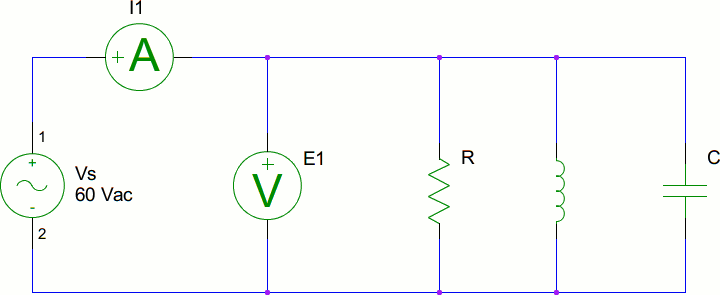
\includegraphics[width=.8\textwidth]{test_circuit}
    \caption{Parallel RLC Circuit Configuration}
    \label{test_circuit}
  \end{center}
\end{figure}

\begin{table}[h]
  \begin{center}
    \begin{tabular}{ccc}
      \hline
      R & L & C \\
      $\Omega$ & H & $\mu$F \\
      \hline
      1200 & 0.8 & --- \\ 1200 & 0.8 & 2.2 \\ 1200 & 0.8 & 4.4 \\
      1200 & 0.8 & 8.8 \\ 1200 & 1.6 & --- \\ 1200 & 1.6 & 2.2 \\
      1200 & 1.6 & 4.4 \\ 1200 & 1.6 & 8.8 \\
      \hline
    \end{tabular}
    \caption{RLC Values for circuit in Figure~\ref{test_circuit}}
    \label{testc_dat}
  \end{center}
\end{table}

\section{Procedure}
Sed luctus lacinia sollicitudin. Praesent arcu sapien, accumsan et convallis
quis, fringilla vel ligula. Morbi id purus massa. Aliquam ut leo tellus, vel
auctor urna. Nulla molestie tellus et velit aliquet convallis.

Suspendisse fermentum tincidunt lorem in pellentesque. Vestibulum tincidunt
nibh eget lectus posuere ut luctus libero pretium. Integer sit amet purus ac
nibh dictum elementum. Quisque sagittis leo eu felis mollis vitae interdum
metus mattis. Maecenas et sem libero.

Vestibulum ante ipsum primis in faucibus orci luctus et ultrices posuere
cubilia Curae; Morbi imperdiet, odio id scelerisque euismod, lectus libero
eleifend justo, sit amet porttitor diam est eget orci. Praesent congue
facilisis sem nec condimentum. Suspendisse mi enim, pharetra imperdiet congue
nec, tincidunt a tellus.

Maecenas lacus risus, elementum a pulvinar vel, ullamcorper a diam. Maecenas
malesuada, turpis sit amet euismod posuere, lectus elit bibendum magna, a
molestie erat neque ut magna. Integer magna neque, ultricies vitae eleifend ac,
mollis eget erat. Aenean risus enim, venenatis quis dapibus vel, ullamcorper id
ante. Proin eget mattis magna. Integer rhoncus facilisis leo eget semper.
Aenean sodales sagittis eleifend. Nulla hendrerit nunc vel felis rutrum
tristique. 

Quisque posuere ullamcorper arcu. Etiam consequat accumsan elit at
semper. Proin vulputate iaculis interdum. Praesent ac enim in enim commodo
malesuada. Quisque non augue at nunc vulputate scelerisque id quis nisi.
Vestibulum id augue eget neque semper aliquet.

Aliquam laoreet elit quis arcu dignissim vitae ornare enim consequat. Donec
sodales dignissim commodo. Vivamus porttitor laoreet tincidunt. Curabitur
aliquam luctus sapien quis tincidunt. Quisque in diam velit, nec luctus nulla.
Mauris vel est nec metus luctus suscipit. Vestibulum mattis laoreet ipsum eu
ullamcorper. Maecenas sit amet tempus nisl. Quisque ut dui at erat dictum
imperdiet. 

Ut aliquet, mi quis tincidunt posuere, eros purus egestas diam, ac
hendrerit quam lectus in orci. Vestibulum ante ipsum primis in faucibus orci
luctus et ultrices posuere cubilia Curae; Proin vulputate porta mauris, ac
congue tortor porta euismod. Donec sit amet massa diam. Etiam sed mi eros,
porta congue libero. Lor

\begin{enumerate}{}{}
  \item Enough description that someone familiar with basic electrical
    measurements could reproduce the experiment.
  \item Sequential
  \item Paragraph form is usually preferred.
  \item Write in past tense.
  \item Do not just copy the instruction lists in the lab assignments.
  \item Learn to be brief
\end{enumerate}

\section{Calc}
\begin{table}[h]
  \begin{center}
    \begin{tabular}{cccccccccc}
      \hline
      R & L & C & I$_1$ & E$_1$ & P & $\theta$ & S & Q & p.f. \\
      $\Omega$ & H & $\mu$F & A & V & W & $\circ$ & VA & VAR & \\
      \hline
      1200 & 0.8 & --- & 0.210 & 60 & 4.56 &  68.77 & 12.58 & 11.73 & 0.36 \\
      1200 & 0.8 & 2.2 & 0.164 & 60 & 4.56 &  62.48 &  9.86 &  8.75 & 0.46 \\
      1200 & 0.8 & 4.4 & 0.122 & 60 & 4.56 &  51.65 &  7.34 &  5.76 & 0.62 \\
      1200 & 0.8 & 8.8 & 0.076 & 60 & 4.56 &  -2.67 &  4.56 & -0.21 & 1.00 \\
      1200 & 1.6 & --- & 0.114 & 60 & 3.39 &  60.27 &  6.84 &  5.94 & 0.50 \\
      1200 & 1.6 & 2.2 & 0.075 & 60 & 3.39 &  41.06 &  4.50 &  2.96 & 0.75 \\
      1200 & 1.6 & 4.4 & 0.057 & 60 & 3.39 &  -0.50 &  3.39 & -0.03 & 1.00 \\
      1200 & 1.6 & 8.8 & 0.115 & 60 & 3.39 & -60.51 &  6.89 & -6.00 & 0.49 \\
      \hline
    \end{tabular}
    \caption{Calculated Data}
    \label{calc_dat}
  \end{center}
\end{table}

\[\mathbf{P} = \mathbf{VI}\cos\theta \]
\[\mathbf{Q} = \mathbf{VI}\sin\theta\]
\[\mathbf{S} = \mathbf{VI}^*\]
\[\mathbf{V} = \mathbf{IZ}\]
\[\text{p.f.} = \cos\theta\]

\section{Results}
\begin{table}[h]
  \begin{center}
    \begin{tabular}{cccccccccc}
      \hline
      R & L & C & I$_1$ & E$_1$ & P & $\theta$ & S & Q & p.f. \\
      $\Omega$ & H & $\mu$F & A & V & W & $\circ$ & VA & VAR & \\
      \hline
      1200 & 0.8 & --- & 0.206 & 60.9 & 4.53 &  68.0 & 12.55 & 11.21 & 0.37 \\
      1200 & 0.8 & 2.2 & 0.158 & 60.9 & 4.56 &  60.9 &  9.62 &  8.19 & 0.49 \\
      1200 & 0.8 & 4.4 & 0.117 & 60.9 & 4.59 &  49.0 &  7.13 &  5.28 & 0.66 \\
      1200 & 0.8 & 8.8 & 0.081 & 61.0 & 4.65 &  -4.4 &  4.94 & -0.36 & 1.00 \\
      1200 & 1.6 & --- & 0.116 & 61.0 & 3.94 &  55.4 &  7.08 &  0.37 & 1.00 \\
      1200 & 1.6 & 2.2 & 0.079 & 61.0 & 3.96 &  32.8 &  4.82 &  2.55 & 0.84 \\
      1200 & 1.6 & 4.4 & 0.067 & 61.0 & 3.99 &  -6.6 &  4.09 & -0.46 & 1.00 \\
      1200 & 1.6 & 8.8 & 0.124 & 61.2 & 4.05 & -57.4 &  7.60 & -6.33 & 0.54 \\
      \hline
    \end{tabular}
    \caption{Experimental Data}
    \label{meas_dat}
  \end{center}
\end{table}

\section{Comparison with Theoretical}
Praesent iaculis metus ornare tellus semper interdum. Nunc cursus sapien quis
tortor condimentum fermentum. Fusce tristique, eros sit amet euismod elementum,
tellus diam porttitor erat, et gravida nisi sapien et orci. Donec nec quam
tempus mi gravida ornare in eu lorem. In sit amet massa vitae ligula malesuada
consectetur. Vivamus faucibus tristique lacus, non scelerisque eros rhoncus ut.
Mauris eget interdum nisi. Nullam ac est odio, in mollis dui. Suspendisse
potenti.

Donec posuere vestibulum viverra. In vestibulum sem nisl. Donec eros tortor,
ultrices a ullamcorper vitae, dapibus ac libero. Vivamus quis nisi elit, non
venenatis urna. Donec porta dolor in ligula vehicula in vulputate ligula
commodo. Donec viverra convallis felis, eget vulputate nunc lacinia eget. 

\begin{enumerate}{}{}
  \item Measured values versus what would be predicted by a theoretical
    analysis of the circuit performance.
  \item For example, compare the measured resistance of two resistors connected
    in series with R$_1 + $R($2$
  \item Express comparison as a \%error.
\end{enumerate}

\[\text{\%deviation} = {\text{measured} - \text{theoretical}} \frac
  {\text{theoretical}} \times \text{100\%}\]

\section{Conclusions}
Pellentesque habitant morbi tristique senectus et netus et malesuada fames ac
turpis egestas. Duis dui turpis, convallis ac hendrerit in, facilisis sed
lectus. Nulla facilisi. Aenean id nulla ante, sit amet venenatis eros.

Fusce orci nibh, pharetra id bibendum sit amet, porta id metus. Sed faucibus
ultricies ullamcorper. Class aptent taciti sociosqu ad litora torquent per
conubia nostra, per inceptos himenaeos. Suspendisse bibendum vestibulum metus
pellentesque gravida. Proin justo ligula, ultrices at faucibus at, blandit ut
libero. Fusce cursus commodo nisl, sit amet pretium velit dignissim quis. Cras
ut posuere felis.

Proin suscipit porta sodales. Sed non massa sit amet dui condimentum convallis.
Vestibulum vitae tincidunt dui. Mauris tincidunt, neque vel congue ornare, sem
sapien eleifend urna, sit amet dictum neque orci id felis. Cras diam nunc,
viverra interdum aliquam sit amet, blandit quis libero. Nunc eget odio
scelerisque eros placerat auctor. Aliquam mattis tellus sed lacus sodales id
molestie risus cursus.

\begin{enumerate}{}
  \item What theoretical principle or concept did this experiment prove?
  \item Within experimental error, this laboratory exercise has demonstrated that
    the equivalent resistance of two resistors connected in series is equal to the
    sum of the individual values.
\end{enumerate}

\end{document}
